\documentclass[aspectratio=43]{beamer}
% \documentclass[aspectratio=169]{beamer} % proyector 16:9 | Ref:  https://en.wikibooks.org/wiki/LaTeX/Presentations
\usetheme{Boadilla}
\beamertemplatenavigationsymbolsempty %% Sin barra navegación
\usecolortheme{beaver}


%% Spanska!
\usepackage[utf8]{inputenc}
\usepackage{lmodern} % no producia letras en matemático | Ref: https://tex.stackexchange.com/questions/250413/error-when-using-greek-symbol-in-subscript-in-beamer-presentation 
\usepackage[spanish]{babel}
\def\spanishoptions{argentina}

%% inclusión de gráficas
\usepackage{graphicx}	% instalar ghostscript-x para que el dvi muestre los eps
\graphicspath{ {./graphs/} {../figuras/} }
\usepackage{rotating}	% epígrafe rotado


\begin{document}

\title{Curso de ingeniería centrado en código}
\subtitle{Capitalizando lo desarrollado durante el confinamiento}
\author[vbettachini@unlam.edu.ar]{Bettachini, V.A.}
\institute[]{
	Ingeniería Mecánica, DIIT, UNLaM
}
\date[2023-09-22]{
	V Encuentro \emph{Mejora de las Estratégias Pedagógicas}\\22 de septiembre de 2023
}

\usebackgroundtemplate{
  
\includegraphics[width=\paperwidth, height=\paperheight]{diit_titre_background}
}	% unset background % https://tex.stackexchange.com/questions/201013/how-to-include-a-background-image-to-only-one-page-of-a-beamer-presentation

\begin{frame} 
  \titlepage
\end{frame}

\usebackgroundtemplate{
  
\includegraphics[width=\paperwidth, height=\paperheight]{diit_background}
} %% https://mprnotes.wordpress.com/2009/08/14/changing-background-image-of-latex-beamer/


\begin{frame}
	\frametitle{Adquisición de competencias: un ejercicio del \emph{copy \& paste}}
	\begin{block}{}
	  \begin{columns}[b]
			\begin{column}{0.3\textwidth}
				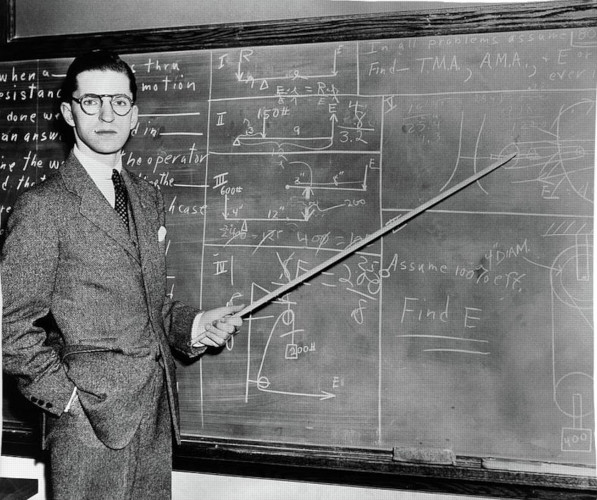
\includegraphics[width= \columnwidth]{1930s-1940s-man-teacher-professor-vintage-images}
			\end{column}
			\begin{column}{0.65\textwidth}
				s. XIX: únicas herramientas pizarrón + papel
				\pause
				\begin{itemize}[<+->]
					% \item Alumnos y docentes pierden tiempo (y se aburren) copiando una y otra vez las mismas cosas
					\item Profesor: \textbf{cada} clase transcribe (o presenta)
					% 	teoría y ejemplos de resolución al 
					\item Alumno: pizarrón (\emph{Powerpoint}) \(\rightarrow\) cuaderno
					\item Resuelto en papel \(\implies\) debe \textbf{transcribirse}
					\item Modelado y cálculos: se \textbf{reiteran}
				\end{itemize}
			\end{column}
		\end{columns}
	\end{block}

	\pause
	\begin{block}{}
	  \begin{columns}[b]
			\begin{column}{0.3\textwidth}
				\includegraphics[width= \columnwidth]{"Screenshot 2023-09-18 at 12-24-03 Google Colaboratory"}
			\end{column}
			\begin{column}{0.65\textwidth}
				s. XXI: minimizar el tedio
				\begin{itemize}[<+->]
					% \item Alumnos y docentes pierden tiempo (y se aburren) copiando una y otra vez las mismas cosas
					\item Profesor: actualiza código en repositorio
					\item Alumno: repositorio del curso \(\rightarrow\) propio
					\item Código modificable \(\implies\) \textbf{re-utilizable} 
					\item Modelado y cálculos: \textbf{única vez}
				\end{itemize}
			\end{column}
		\end{columns}
	\end{block}
\end{frame}


\begin{frame}
	\frametitle{Los futuros ingenieros deben poder escribir código}
	\pause
	\begin{block}{}
		\begin{itemize}[<+->]
			\item Usan calculadora pues \textbf{aprendieron} aritmética en la primaria.
			\item Usarán álgebra computacional pues \textbf{aprobaron} álgebra y análisis.
			\begin{itemize}[<+->]
				\item Enfocarse en nuevas habilidades, no en cálculos automatizables.
				%\item Álgebra y análisis simbólico
				\item Con cálculo numérico resolverán lo imposible en pizarrón/papel.
			\end{itemize}
			\item Enfoque constructivista de la re-utilización del código
			\begin{itemize}[<+->]
				\item El código inicial es provisto por el docente.
				\item Modificaciones aditivas resuelven nuevas problemáticas.
				\item Alumno se torna autónomo reutilizando el propio.
			\end{itemize}
		\end{itemize}
	\end{block}
		% \uncover<4->{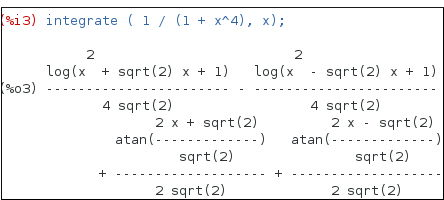
\includegraphics[height= 2cm]{ucarecdn}}
		\only<2>{\includegraphics[height= 2cm]{reglacalculadora}}
		\uncover<3->{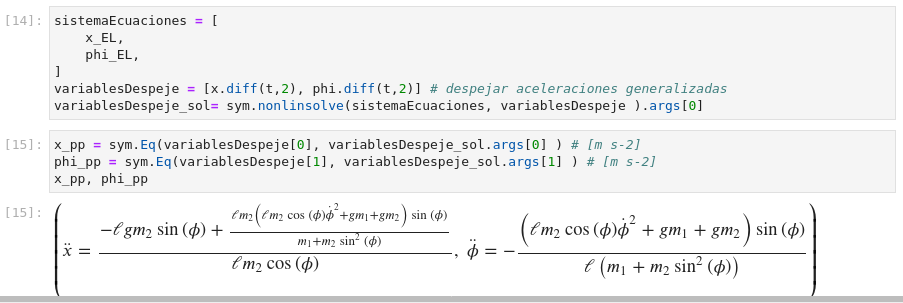
\includegraphics[width= 0.49\textwidth]{hard}}
		\uncover<5->{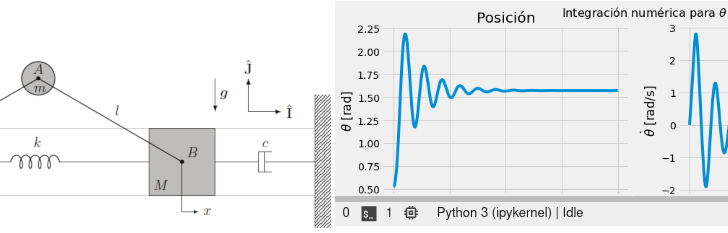
\includegraphics[width= 0.49\textwidth]{impracticable}}
\end{frame}


\begin{frame}
	\frametitle{s.XXI: todo material debe estar disponible en línea}
	\pause
	\begin{block}{Cuaderno programable en línea: texto + ecuaciones + código}
		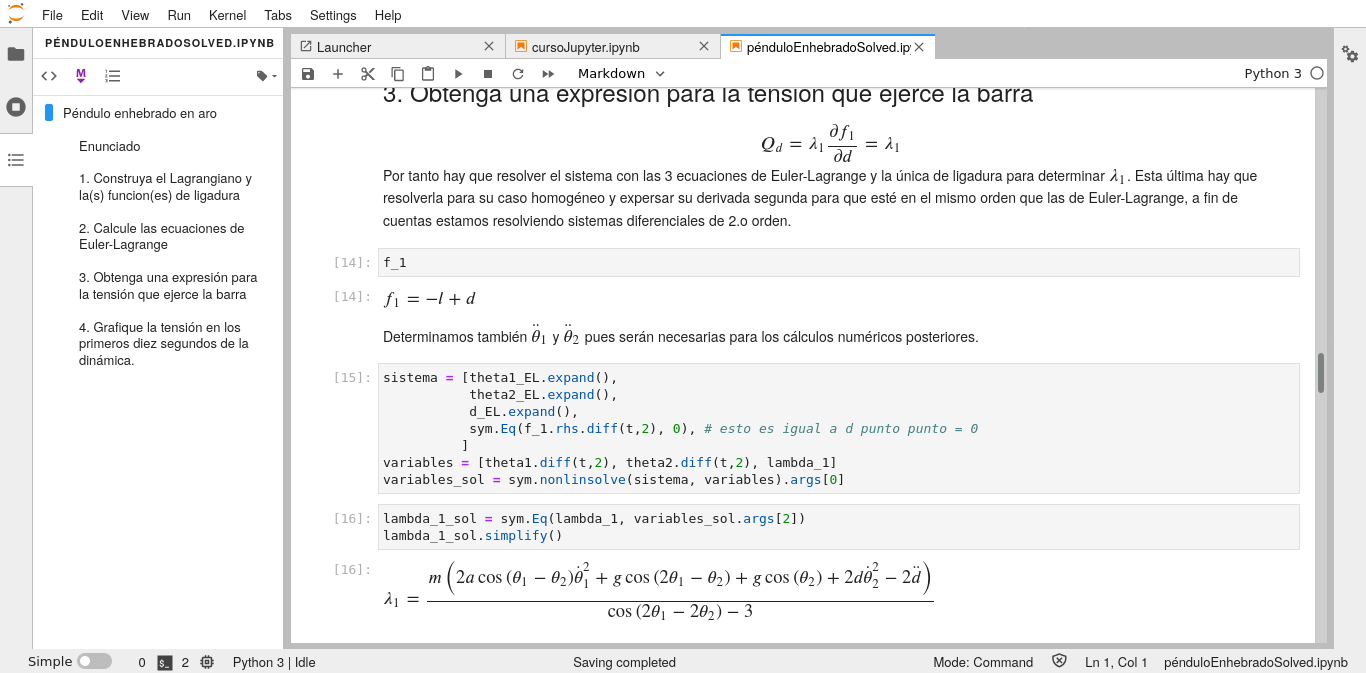
\includegraphics[width= \columnwidth]{screenshot_JupyterLab}
	\end{block}
\end{frame}


\begin{frame}
	\frametitle{Cursada centrada en el código}
	\begin{block}{Teoría y ejercicios resueltos en cuadernos programables}
		\begin{itemize}[<+->]
			\item En línea se distribuye la teoría y se resuelven ejercicios.
			\item Modificando el código se resuelven guías semanales de ejercicios.
			\item Se asiste a los alumnos con consultas asincrónicas.
			% \item Se responzabiliza al alumno con la primer lectura de la teoría.
			\item Cuadernos multi-usuario, se incentiva el trabajo remoto colaborativo.
			\item Todos sus ejercicios tienen fecha límite de entrega para su corrección.
		\end{itemize}
	\end{block}

	\pause
  \begin{columns}[b]
    \begin{column}{0.35\textwidth}
			\begin{block}{Aula invertida}
				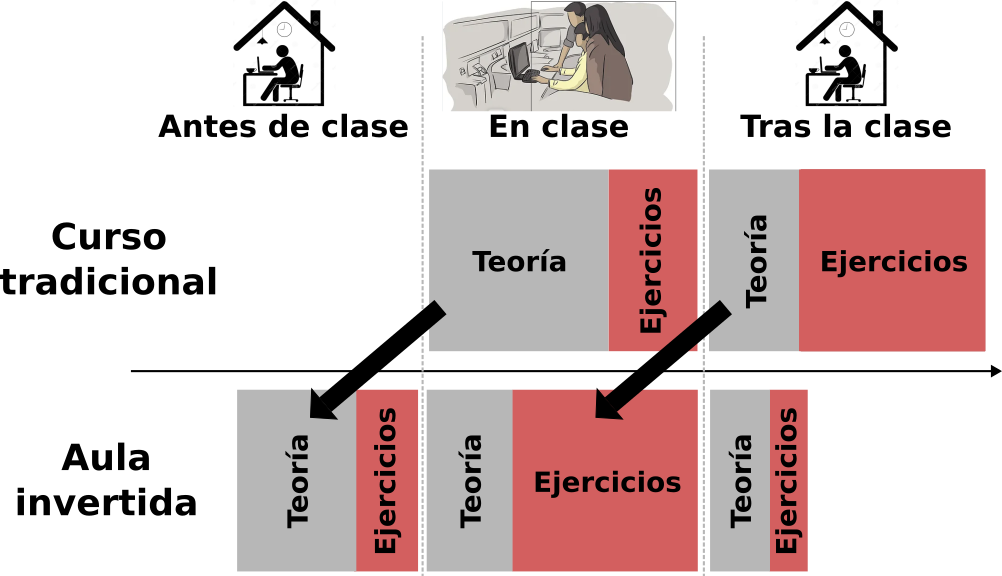
\includegraphics[width= \columnwidth]{diagramaTiempo2.png}
			\end{block}
    \end{column}
    \begin{column}{0.6\textwidth}
			\begin{block}{}
				\begin{tabular}{lll}
					\hline
					Sincrónico & Teoría & Ejercicios\\
					\hline
					Antes & Leer y aplicar & Iniciarles\\
					Durante & Aclarar dudas & Terminarles\\
					% Durante & Aclarar dudas & \begin{tabular}{@{}c@{}}Terminarles\\(semanal)\end{tabular}\\
					Luego & \begin{tabular}{@{}c@{}}Consultas\\adicionales\end{tabular} & \begin{tabular}{@{}c@{}}Correcciones\\del docente\end{tabular}\\
					\hline
				\end{tabular}
			\end{block}
    \end{column}
  \end{columns}
\end{frame}



\begin{frame}
	\frametitle{Asistencia docente y corrección asincrónica}
	\begin{block}{Google Colaboratory: comentando y editando el ejercicio del alumno}
		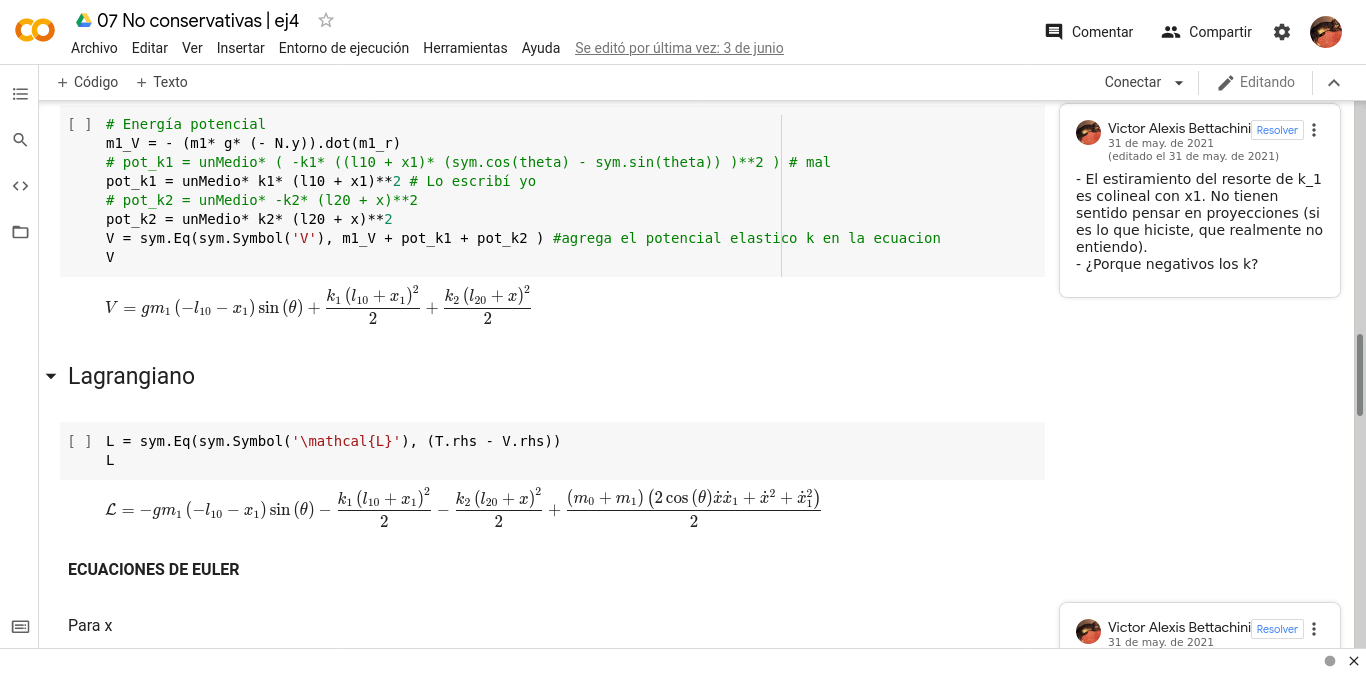
\includegraphics[width= \columnwidth]{comentariosColab}
	\end{block}
\end{frame}


\begin{frame}
	\frametitle{Seguimiento individualizado}
	\begin{block}{Registro del cumplimiento con entregas semanales}
		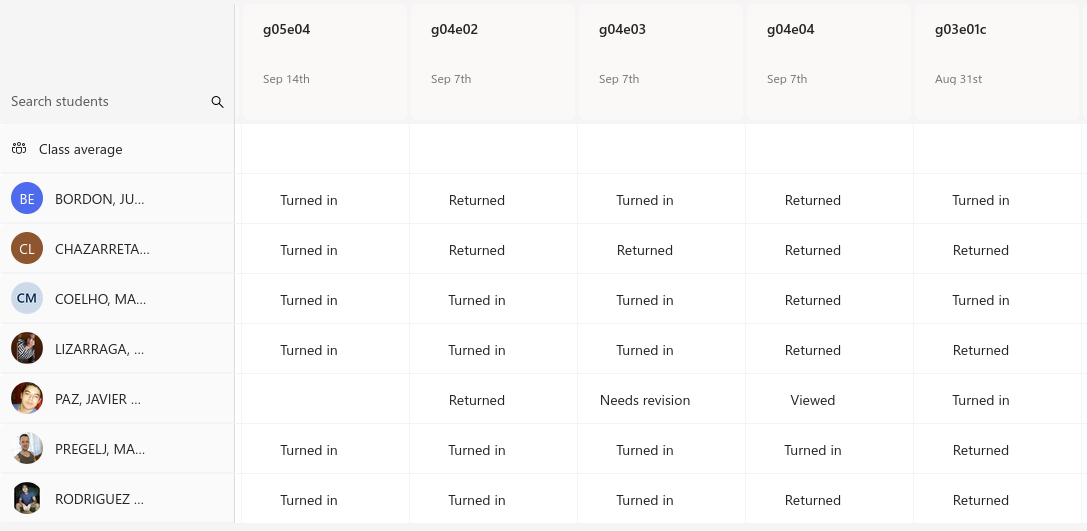
\includegraphics[width= \columnwidth]{seguimiento}
	\end{block}
\end{frame}




\begin{frame}
	\frametitle{Actualidad del proyecto}
	\pause
	\begin{block}{}
		\begin{description}[<+->]
			\item [2023] Retro-alimentación de los alumnos mejoró:
				\begin{itemize}
					\item Apuntes y código en el repositorio.
					\item Metodología ejercitación y evaluación.\\
							Mayor exigencia de ejercicios \(\rightarrow\) mejor respuesta.
				\end{itemize}
			\item [2024] 
				\begin{itemize}
					\item Física II empleará simulaciones provistas por nosotros.
					\item \emph{Prompt engineering}: alumnos generarán código con IA.
				\end{itemize}
			% \item [202x] Difundir la metodología en el DIIT.
		\end{description}
	\end{block}
	\uncover<6->{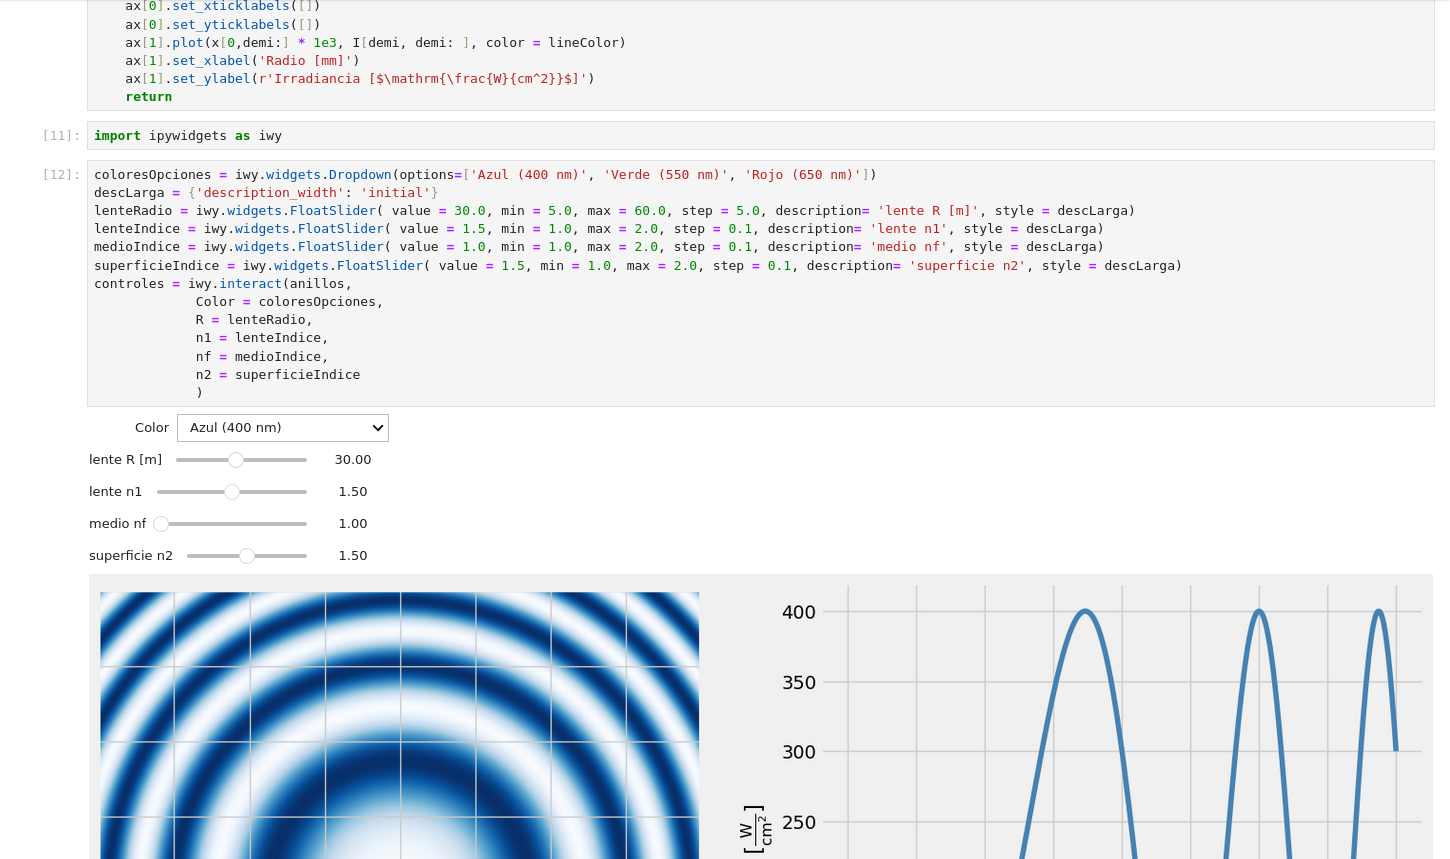
\includegraphics[height= 3cm]{cuñaAnillosN}}
	\uncover<7->{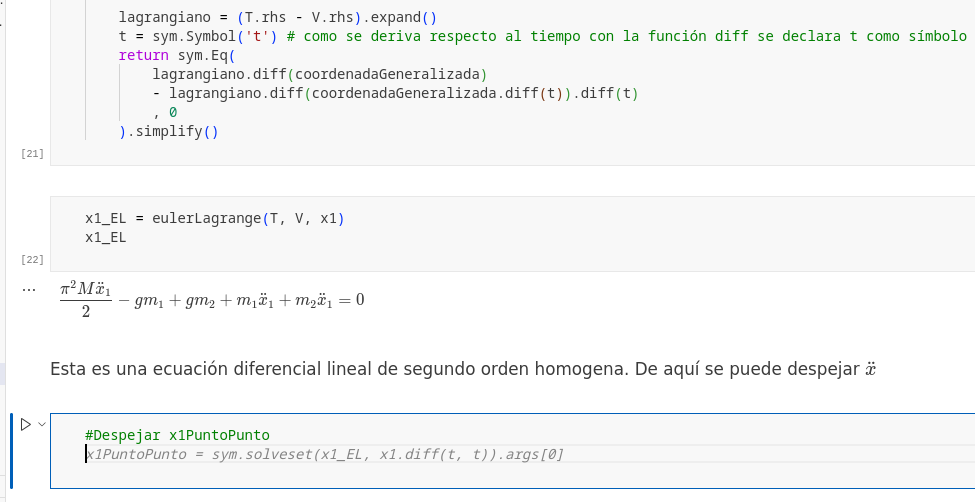
\includegraphics[height= 3cm]{copilot}}
\end{frame}


\end{document}
